\section{A Framework for Assessing Static and Dynamic Personalization}\label{ss:framework}

In this section, we present the components of our framework for assessing static and dynamic personalization, including details for fitting a heirarchical Bayesian PK model to concentration data from a cohort of patients, assessing the behaviour of markov chains via diagnostics, and using the Bayesian model to generate simulated data for evaluation. We then outline several modes of static and dynamic personalization ranging from no personalization (every patient gets the same dose) to a complex dynamic mode of personalization (estimation of the optimal policy for dosing from a dynamic treatment regime).  Finally, we outline steps for assessing the benefits of each mode of personalization.

\subsection{Bayesian Modelling}

The first step in our framework is to fit a Bayesian model that relates patient covariates and dose to drug concentration as a function of time. For example, previous work \cite{pananos2020comparisons} describes a hierarchical Bayesian model of apixaban pharmacokinetics, in which the clearance rate (L/hour), time to max concentration (hours), absorption time delay (hours), and ratio between the elimination and absorption rate constants (called alpha, a unitless parameter) are hierarchically modelled. In our case study, we extend that model by regressing the latent pharmacokinetic parameters on baseline clinical variables (age, sex, weight, and creatinine) to permit personalization. The model could equally well be extended with pharmacokinetic or biomarker information if the relevant theory and data were available for a particular use case.

Once the form of the model is specified, creating simulated patients or estimating the PK parameters of a real patient requires computation of or sampling from the posterior distribution of the relevant variables given the relevant data. However, exact computation of the posterior distribution is intractable for all but very simple models, so Markov chain Monte Carlo (MCMC) techniques are often used to approximate the expectations with respect to the posterior distribution.  Presently, the gold standard for generating samples from the posterior is Hamiltonian Monte Carlo (HMC), which works by generating a sequence of samples that ``explores'' the space of possible sampled values in a way that reflects the posterior distribution.  Many implementations of HMC come with diagnostics which monitor the behaviour of the Markov chains that are used to generate samples and help to ensure that they are representative of the posterior distribution. That these Markov chains behave well is crucial, as any inferences about or from the model are obtained from samples generated by the chains. To assess the quality of the markov chains, several diagnostics are commonly used including: number of divergences, the Gelman-Rubin convergence diagnostic, and effective sample size \cite{betancourt2018conceptual}.

In practice, several Markov chains are used simultaneously to generate samples from the posterior. The chains are assessed with within-chain and between-chain diagnostics. First, individual chains may sometimes \textit{diverge}. A divergence in a Markov chain indicates that the HMC Markov chain has encountered a region of high curvature in the posterior distribution which cannot be adequately explored.  Consequently, Monte Carlo estimators of any expectations can be biased due to incomplete exploration of the posterior distribution.  It is important that none of the Markov chains generated by HMC display a divergence, and that many chains (typically 4 or more) are initialized and are allowed to explore the posterior distribution. 

Having ensured that no chains are diverging, a group-level diagnostic is used to assess whether all chains have converged to the same limiting distribution.  The \textit{Gelman-Rubin (sometimes called $\hat{R}$) convergence diagnostic} is designed to detect if the Markov chains have converged to the same distribution by measuring the within-chain variance to the between chain-variance. In practice, $1.05<\hat{R}$ indicates that there is poor mixing of the Markov chains and inference from the samples should not be performed lest the Monte Carlo estimators are biased by this poor mixing.

Even if the chains do not exhibit divergences and arrive at the same limiting distribution, the Markov chains could still exhibit high within-chain correlation, thereby increasing the uncertainty of estimation of key posterior quantities such as means, variances, or quantiles \cite{brooks2011handbook}.  The \textit{effective sample size} is a measure of how much the within chain autocorrelation increases uncertainty estimates.  In some software packages, the effective sample size is reported as a fraction of the total number of samples drawn from the Markov chains.  Presently, the guidance is that the effective sample size ratio should be no smaller than 1\%.



In addition to monitoring divergences, Gelman-Rubin convergence diagnostics, and effective sample sizes, the model should be evaluated against existing domain knowledge.  Evaluating that the model has learned appropraite behaviour (e.g. that as one quantity increases, another should decrease) can be performed by plotting model predictions.  Additionally, \textit{posterior predictive checks} -- generating synthetic data  from the model's posterior distirbution and comparing against the real data -- can be performed to ensure the model is not generating data which are physically impossible or completely unrealistic. Once the model is fit, important diagnostics indicate no pathalogical behaviour, and the model is deemed to fit the data sufficiently well, the model can then used to generate synthetic pharmacokinetic data for use in experiments to compare different forms of personalization. Each generated data point may be thought of as one synthetic patient, with observed covariates and observed pharmacokinetic parameters. These parameters, which are never observed in real data, allow us to compute the effects of any dosing decisions (which are made \textit{without} direct knowledge of the parameters), and thus allow us to evaluate the performance of different modes of personalized dosing on the sampled population. 

\subsection{Modes of Personalization}

The second step in our framework is to identify modes of personalization that we wish to evaluate. We classify these modes of personalization into two types: static and dynamic personalization.

Static modes of personalization seek to inform the dose at one point in time (usually induction) with the goal of eliminating the need for ``trial-and-error'' adjustments.  We consider two modes of static personalization in our case study:

\begin{enumerate}
	\item \textbf{One size fits all}.  This mode of personalization is not very personal at all.  All patients receive the same dose size at the onset of treatment.
	\item \textbf{Dose based on clinical variables}.  In this mode of personalization, the patient's covariates, for example age, sex, weight, creatinine measurements, and possibly genetic or biomarker information, are provided to the pharmacokinetic model.  A dose size is then selected using the model to maximize the reward function conditional on these measurements.
\end{enumerate}

\noindent Dynamic modes of personalization seek to personalize the initial doses but also the titration process.  We consider four modes of dynamic personalization for our case study:

\begin{enumerate}
	\item \textbf{One size fits all initial dose \textit{and} one dose adjustment}.  This mode of personalization provides patients the same dose to start, but requires a concentration measurement to be made sometime in the future, which is then used to adjust the dose.  For example, in our case study, subjects take their initial dose once every 12 hours with perfect adherence for five days.  Our pharmacokinetic model conditions on this measurement, and the dose is adjusted in order to maximize the reward for another five days.
	
	\item \textbf{Initial dose based on clinical variables \textit{and} one dose adjustment}.  Here, the initial dose provided to the patient is determined by the patient's clinical measurements. For example, in our case study, in the second half of the fifth day, a concentration measurement is made at a random time. The model is conditioned on this concentration and the dose is adjusted to optimize the reward.
	
	\item \textbf{Initial dose based on clinical variables \textit{and} optimally-timed dose adjustment}.  Similar to the previous mode of personalization, but the time at which the measurement is made is under our control and tuned to maximize reward. The time at which the sample is taken can yield more or less information about particular parameters in the model. For example, much later after the dose is taken yields more information about the elimination rate constant $k_e$ than it does about the absorption rate constant $k_a$ because later in time, the majority of the dose has been absorbed and is now being eliminated by the body. In this mode of personalization, the initial dose and the timing of the adjustment are optimized independently. 
	
	\item \textbf{Optimal sequential dosing policy}. The approach of this mode is the same as the previous mode, except that the initial dose and the timing of the adjustment are \textit{jointly optimized} using Q-learning to maximize the expected reward.
\end{enumerate}

Here, we stress that these are just examples of some modes of personalization, and that we do not mean that these modes should always be candidate modes for personalization, nor that they are the only modes of interest.  These modes may not be appropriate for all drugs across all clinics, and were selected in order to illustrate natural extensions and combinations of static personalization with additional information collection. A strength of our approach is that many possible modes of personalization may be considered depending on what is appropriate for the use-case at hand.

\subsection{Evaluation}

To evaluate the potential for personalization, we compare all of the modes identified in step 2 based on their achieved reward as well as the difference between the achieved reward and theoretically largest reward the reward we would achieve if we knew each patient's pharmacokinetic parameters exactly. Because we know the true latent pharmacokinetic parameters of the simulated subjects, we can optimize the reward with the known pharmacokinetics of the subject, thereby yielding the largest reward possible.

In reality, at the time of dose adjustment, the actual reward is not known.  However, because a Bayesian model is a generative model, samples generated from that model can be used to compute the expected reward achieved by any choice of dose.  The steps for computing the expected reward for a given dose are as follows:

\begin{enumerate}
	\item Condition the model on available patient information if the mode of personalization permits. For some modes of personalization, this might be clinical measurements, blood concentration measurements, both, or neither.
	
	\item Draw several sets of of pharmacokinetic parameters from the posterior distribution. Each of these sets represents a possible underlying truth for the patient  under consideration. Choosing one of these sets of pharmacokinetic parameters as ``the truth'', in conjunction with the dose schedule considered, completely determines the concentration profile and allows us to make a prediction of the patient's concentration into the future. Each set of parameters thus corresponds to a concentration, resulting in a distribution over possible future trajectories of concentrations.
	
	\item Compute the concentration profile on a grid of times.  The grid must be sufficiently fine to capture changes in the concentration over time.  We make a prediction at 15 minute intervals.
	
	\item Compute the reward for the proposed dose based on the resulting concentration trajectory.
	
	\item Update the proposed dose and recompute the reward.
\end{enumerate}

The concentration profile scales linearly with dose size; double the dose, double the concentration at a given time.  This relationship allows for off-the-shelf optimizers to be used in the selection of dose size in this process.

\begin{figure}
	\centering
	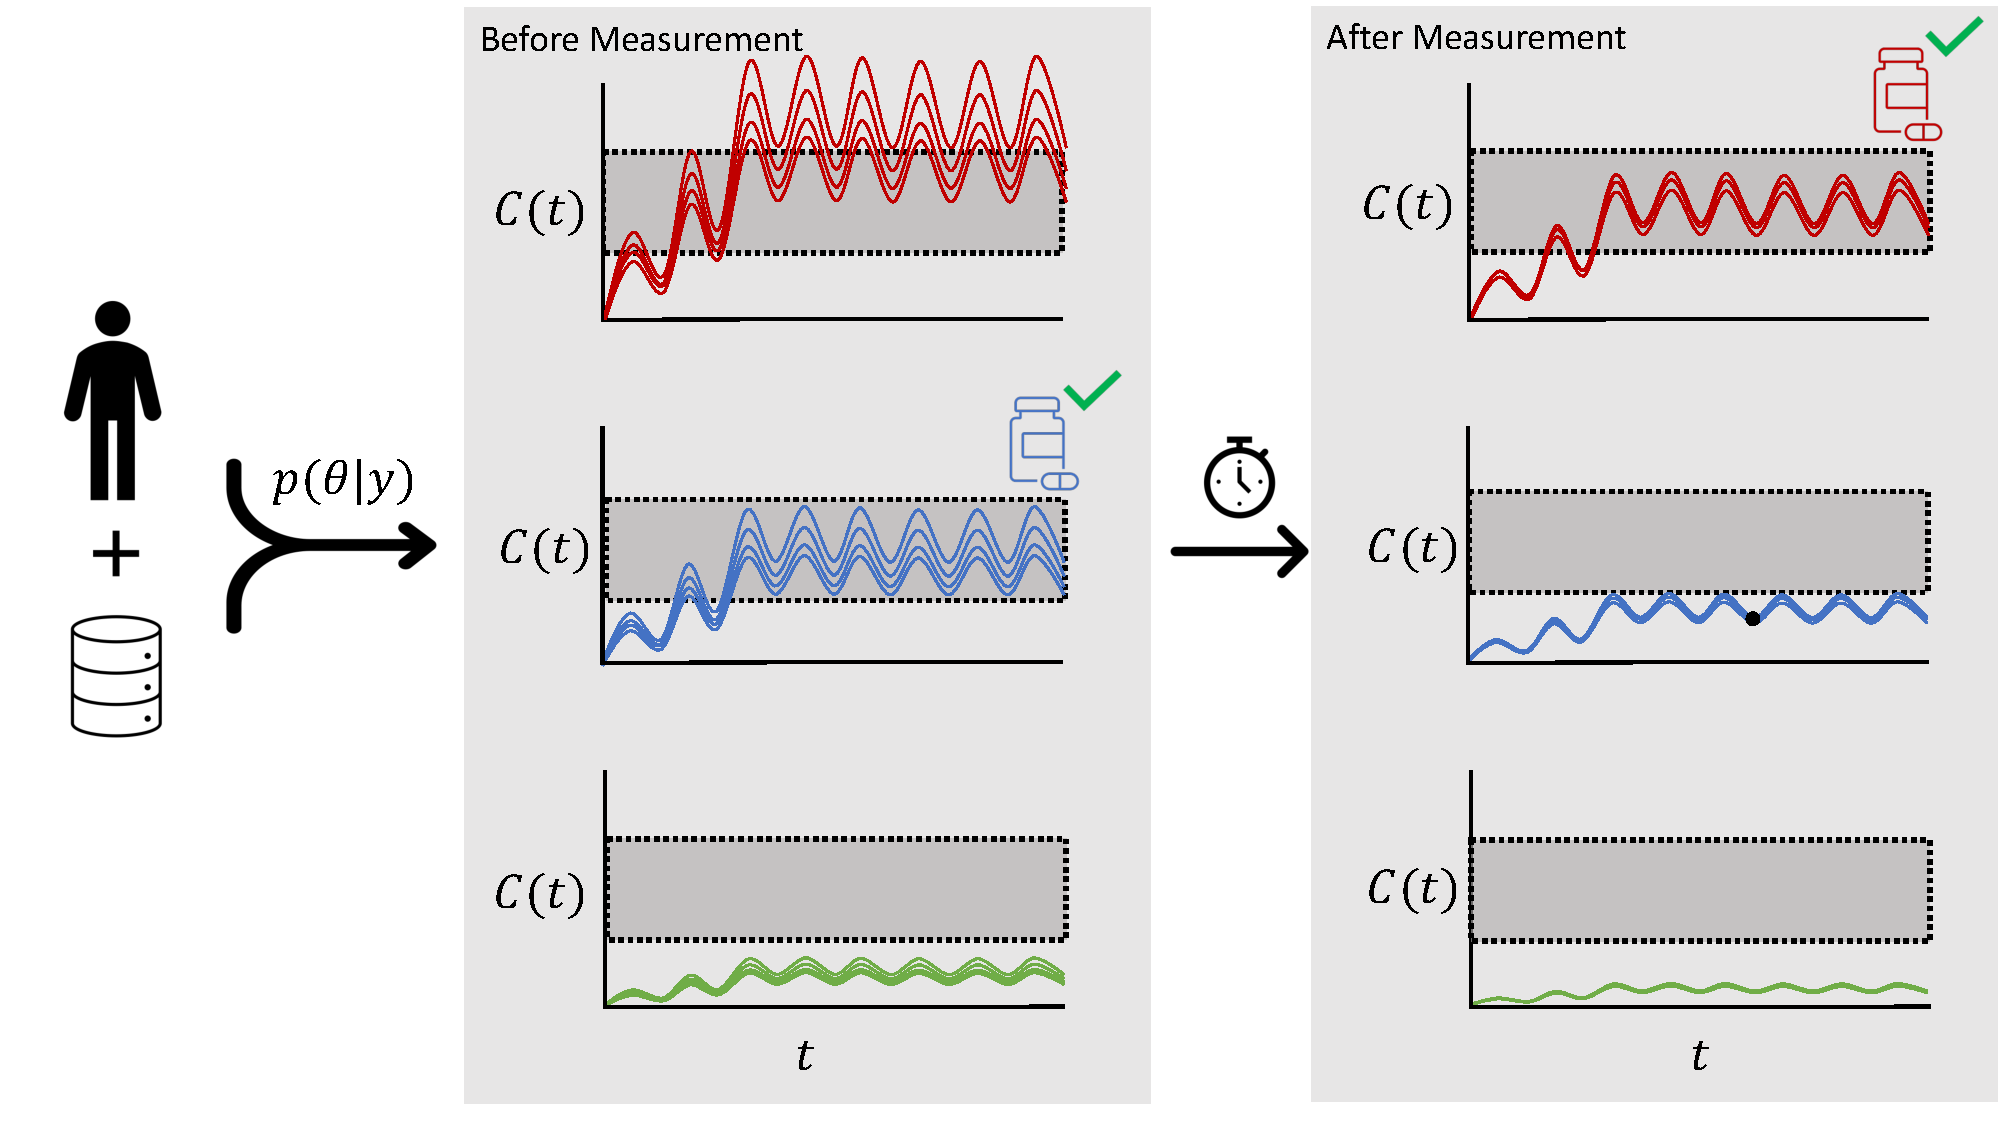
\includegraphics[width=0.85\linewidth]{figures/process_figure_single}
	\caption{Illustration of our framework.  Intelligent caption here.}
	\label{fig:processfiguresingle}
\end{figure}

